% !TEX TS-program = xelatex
\documentclass[aspectratio=169]{beamer}

% --- THEME & LAYOUT ---
\usetheme[numbering=fraction,progressbar=head]{metropolis}
\setbeamersize{text margin left=8mm,text margin right=8mm}

% --- CUSTOM FOOTER WITH TLP MARKING ---
\setbeamertemplate{frame footer}{\textbf{TLP:CLEAR} -- L'information peut \^etre partag\'ee librement sans restriction.}
\setbeamercolor{frame footer}{fg=cyber-accent}

\usepackage{amsmath}

% --- FONTS (XeLaTeX) ---
\usepackage{fontspec}
\setsansfont[
  Ligatures=TeX, Scale=1.02,
  BoldFont = {IBM Plex Sans Bold},
  ItalicFont = {IBM Plex Sans Italic}
]{IBM Plex Sans}
\setmonofont{IBM Plex Mono}

% --- ICONS ---
\usepackage{fontawesome5}

% --- COLORS (cyber palette) ---
\definecolor{cyber-bg}{HTML}{0B0F14}
\definecolor{cyber-ink}{HTML}{E6EEF5}
\definecolor{cyber-accent}{HTML}{217EAA}
\definecolor{cyber-mid}{HTML}{7D9CB7}
\definecolor{cyber-soft}{HTML}{8CA4AC}
\setbeamercolor{normal text}{fg=cyber-ink,bg=cyber-bg}
\setbeamercolor{frametitle}{fg=cyber-ink,bg=cyber-bg}
\setbeamercolor{progress bar}{fg=cyber-accent,bg=cyber-soft}
\setbeamercolor{alerted text}{fg=cyber-accent}

% --- LINKS ---
\hypersetup{colorlinks=true, linkcolor=cyber-accent, urlcolor=cyber-accent}

% --- CODE / BOXES ---
\usepackage{listings}
\lstset{
  basicstyle=\ttfamily\footnotesize,
  backgroundcolor=\color{black!5},
  frame=single, rulecolor=\color{cyber-soft},
  keywordstyle=\color{cyber-accent}\bfseries,
  commentstyle=\color{cyber-soft},
  showstringspaces=false
}
\usepackage[most]{tcolorbox}
\tcbset{colback=black!5!cyber-bg, colframe=cyber-soft, coltext=cyber-ink, boxsep=1mm, left=2mm, right=2mm}

% --- PDF TOOLS ---
\usepackage{pdfpages}

% --- GRAPHICS ---
\usepackage{graphicx}

% --- SPEAKER NOTES ---
\usepackage{pgfpages}
% \setbeameroption{hide notes}
% \setbeameroption{show notes}
% \setbeameroption{show only notes}

% --- SPACING IMPROVEMENTS ---
\setbeamertemplate{itemize/enumerate body begin}{\vspace{-0.5ex}}
\setbeamertemplate{itemize/enumerate subbody begin}{\vspace{-0.5ex}}

% --- TITLE INFO ---
\title{\faIcon{shield-alt}\; Range42 -- Avanc\'ees \& D\'emo en direct}
\subtitle{Plateforme ouverte de cyber range pour la formation collaborative en s\'ecurit\'e}
\author{NC3 / \'Equipe Range42}
\date{FIC Lille 2026}
\institute{\faServer\; Proxmox \quad \faCogs\; Ansible \quad \faProjectDiagram\; Orchestration \quad \faBinoculars\; T\'el\'em\'etrie}

\begin{document}

% === TITRE ===
\begin{frame}[plain,noframenumbering]
  \titlepage
  \note[item]{Objectif : pr\'esentation de 20 minutes sur les avanc\'ees de Range42 depuis 2025 avec d\'emo en direct du deployer UI.}
  \note[item]{Public : professionnels de la cybers\'ecurit\'e, gouvernement, partenaires europ\'eens.}
\end{frame}

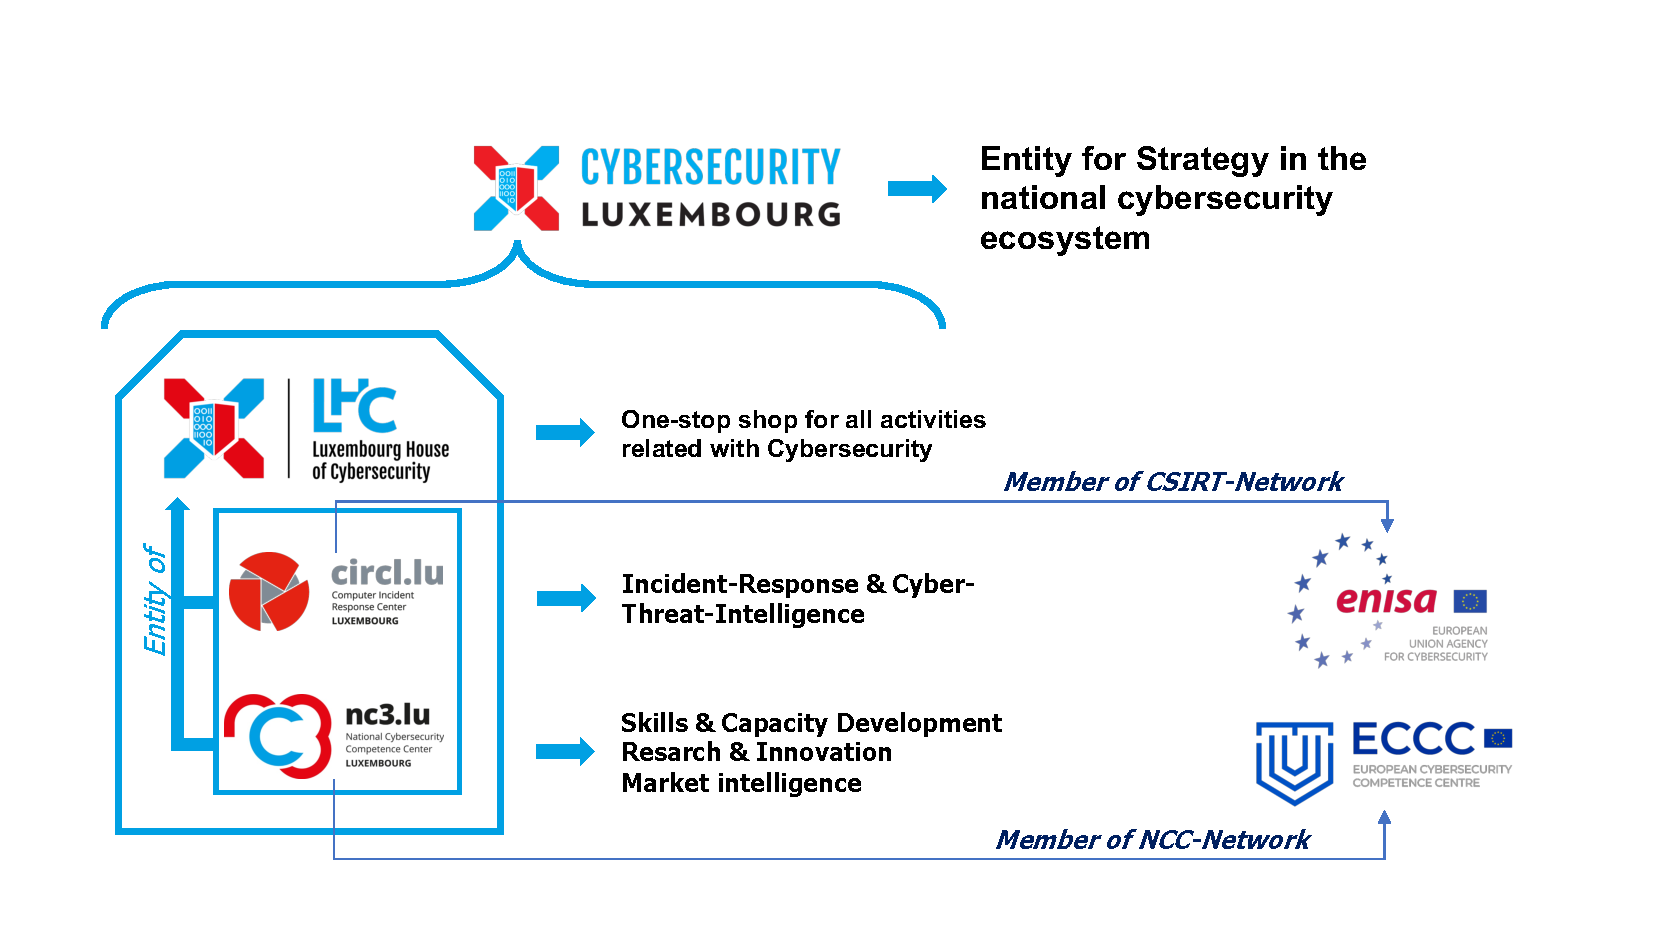
\includepdf[pages={1-2}]{../../pdf_slides/LHC_NC3.pdf}

% === ARGENT PUBLIC, CODE PUBLIC ===
\begin{frame}{Argent public, code public. Allons jusqu'au bout !}
  \begin{columns}[T]
    \column{0.65\textwidth}
    \textbf{\'Equipe \& financement}
    \begin{itemize}
      \item \'Equipe de 3 d\'eveloppeurs -- InfoSec \& DevOps
      \item Mod\`ele collaboratif avec le NC3 \& partenaires
      \item Subvention publique pour l'infrastructure de formation cyber
      \item Mod\`ele FOSS : pas de licence \textcolor{green}{\faMoneyBill}, d\'eveloppement transparent
    \end{itemize}

    \column{0.3\textwidth}
    \vspace{2mm}
    \begin{figure}
      \centering
      
\includegraphics[width=\textwidth]{../../images/logos/FSFE_Public_Money_Public_Code_logo.pdf}
    \end{figure}
  \end{columns}
  \note[item]{Insister sur : financement public = propri\'et\'e publique = b\'en\'efice public.}
\end{frame}

% === AGENDA ===
\begin{frame}{Agenda}
  \begin{enumerate}
    \item Qu'est-ce que Range42 et pourquoi c'est important
    \item Avanc\'ees depuis 2025 : les nouveaut\'es
    \item Vue d'ensemble de l'architecture
    \item \alert{D\'emo en direct} : le Deployer UI en action
    \item Ce qui fonctionne aujourd'hui vs.\ ce qui arrive
    \item Feuille de route : 6 axes strat\'egiques
    \item Comment participer
  \end{enumerate}
  \note[item]{Mettre en avant la d\'emo comme pi\`ece ma\^itresse de la pr\'esentation.}
\end{frame}

% === QU'EST-CE QUE RANGE42 ===
\begin{frame}{Qu'est-ce que Range42 ?}
  \begin{itemize}
    \item \textbf{Plateforme ouverte de cyber range} pour l'entra\^inement offensif, d\'efensif et hybride
    \item \textbf{Infrastructure-as-Code reproductible} : Proxmox, Ansible, Docker
    \item \textbf{Flexible \& extensible} : labs CVE, erreurs de configuration, forensique, analyse de malware
  \end{itemize}
  \begin{tcolorbox}
    \faInfoCircle\; Con\c{c}ue pour simuler des \emph{incidents r\'eels} en toute s\'ecurit\'e, avec isolation, snapshots et t\'el\'em\'etrie.
  \end{tcolorbox}
  \note[item]{Ancrer sur le r\'ealisme s\'ecuris\'e et l'extensibilit\'e.}
\end{frame}

% === AVANC\'EES DEPUIS 2025 ===
\section{Avanc\'ees depuis 2025}

\begin{frame}{Avanc\'ees depuis 2025 \; \faChartLine}
  \textbf{En chiffres}
  \begin{itemize}
    \item \alert{520+ commits} sur 14 d\'ep\^ots (contre 400+ en 2025)
    \item Backend API : 156 commits -- \textbf{refactoring majeur} (86 routes $\rightarrow$ 10 modules)
    \item Deployer UI : 74 commits -- du prototype \`a un \textbf{outil fonctionnel}
    \item Proxmox controller : 112 commits -- cloud-init, templates VM, stockage
  \end{itemize}
  \vspace{1mm}
  \textbf{Jalons cl\'es}
  \begin{itemize}
    \item \alert{D\'eploiement Docker} pour le backend API
    \item \alert{Statut VM en temps r\'eel} via WebSocket sur le canvas
    \item \alert{Suite de tests compl\`ete} et documentation Sphinx
    \item \alert{Article CyCon 2026 soumis} -- publication acad\'emique
  \end{itemize}
  \note[item]{Progr\`es concrets et mesurables.}
\end{frame}

% === R\'EALISATIONS ACTUELLES ===
\begin{frame}{R\'ealisations actuelles \; \faCheckCircle}
  \textbf{Ce qui fonctionne aujourd'hui}
  \begin{itemize}
    \item \alert{$\sim$100 CVE \& erreurs de config identifi\'ees}, $\sim$20 sc\'enarios d\'eployables
    \item \textbf{Provisionnement automatis\'e} sur Proxmox avec r\'eseau, VPN, pare-feu
    \item \textbf{Concepteur visuel de labs} avec composition glisser-d\'eposer
    \item \textbf{Monitoring int\'egr\'e} via Wazuh pour la t\'el\'em\'etrie et les alertes
    \item \textbf{14 d\'ep\^ots} g\'erant automatisation, contenu et outillage
  \end{itemize}
  \vspace{2mm}
  \begin{tcolorbox}
    \faLightbulb\; \textbf{Jalon cl\'e} : le backend est pr\^et pour la production. Le concepteur visuel est d\'esormais fonctionnel et utilis\'e activement.
  \end{tcolorbox}
  \note[item]{Insister : backend ET frontend sont op\'erationnels.}
\end{frame}

% === PAYSAGE CONCURRENTIEL ===
\begin{frame}[shrink=5]{Range42 vs.\ autres cyber ranges}
  \begin{table}
    \tiny\color{cyber-ink}
    \begin{tabular}{l|cccc}
      \textbf{Fonctionnalit\'e} & \textbf{Range42} & \textbf{SaaS commercial} & \textbf{Cloud natif} & \textbf{Traditionnel} \\
      \hline
      \alert{Architecture ouverte} & \checkmark & \texttimes & \texttimes & \texttimes \\
      \alert{IaC/GitOps} & \checkmark & \textasciitilde & \checkmark & \texttimes \\
      D\'eploiement priv\'e & \checkmark & \texttimes & \textasciitilde & \checkmark \\
      Ma\^itrise des co\^uts & \checkmark & \texttimes & \textasciitilde & \checkmark \\
      Souverainet\'e des donn\'ees & \checkmark & \texttimes & \texttimes & \checkmark \\
      Orchestration API & \checkmark & \checkmark & \checkmark & \texttimes \\
      Reset/Snapshots rapides & \checkmark & \checkmark & \textasciitilde & \textasciitilde \\
      Sc\'enarios personnalis\'es & \checkmark & \texttimes & \textasciitilde & \checkmark \\
      \alert{Concepteur visuel de labs} & \checkmark & \checkmark & \texttimes & \texttimes \\
    \end{tabular}
  \end{table}
  \vspace{1mm}
  \begin{tcolorbox}
    \faLightbulb\; \textbf{L'atout Range42} : contr\^ole total, reproductibilit\'e et rentabilit\'e sans d\'ependance fournisseur.
  \end{tcolorbox}
  \note[item]{Le concepteur visuel est un nouveau diff\'erenciateur depuis 2025.}
\end{frame}

% === ARCHITECTURE ===
\begin{frame}[squeeze]{Architecture en un coup d'\oe il}
  \begin{itemize}
    \item \textbf{Couche hyperviseur} : VMs/LXC Proxmox ; snapshots ; segments r\'eseau
    \item \textbf{Couche automatisation} : r\^oles Ansible pour le cycle de vie, r\'eseau, pare-feu, images
    \item \textbf{Plan de contr\^ole} : Backend API (FastAPI) avec Docker ; WebSocket pour le statut en direct
    \item \textbf{Couche UX} : Deployer UI (concepteur visuel), EMP (en d\'eveloppement)
    \item \textbf{Observabilit\'e} : Wazuh pour logs/alertes ; t\'el\'em\'etrie structur\'ee
  \end{itemize}
  \note[item]{Souligner WebSocket et Docker comme nouveaut\'es architecturales.}
\end{frame}

\begin{frame}[shrink=8]{Architecture : composants logiques $\rightarrow$ d\'ep\^ots GitHub}
  \begin{figure}
    \centering
    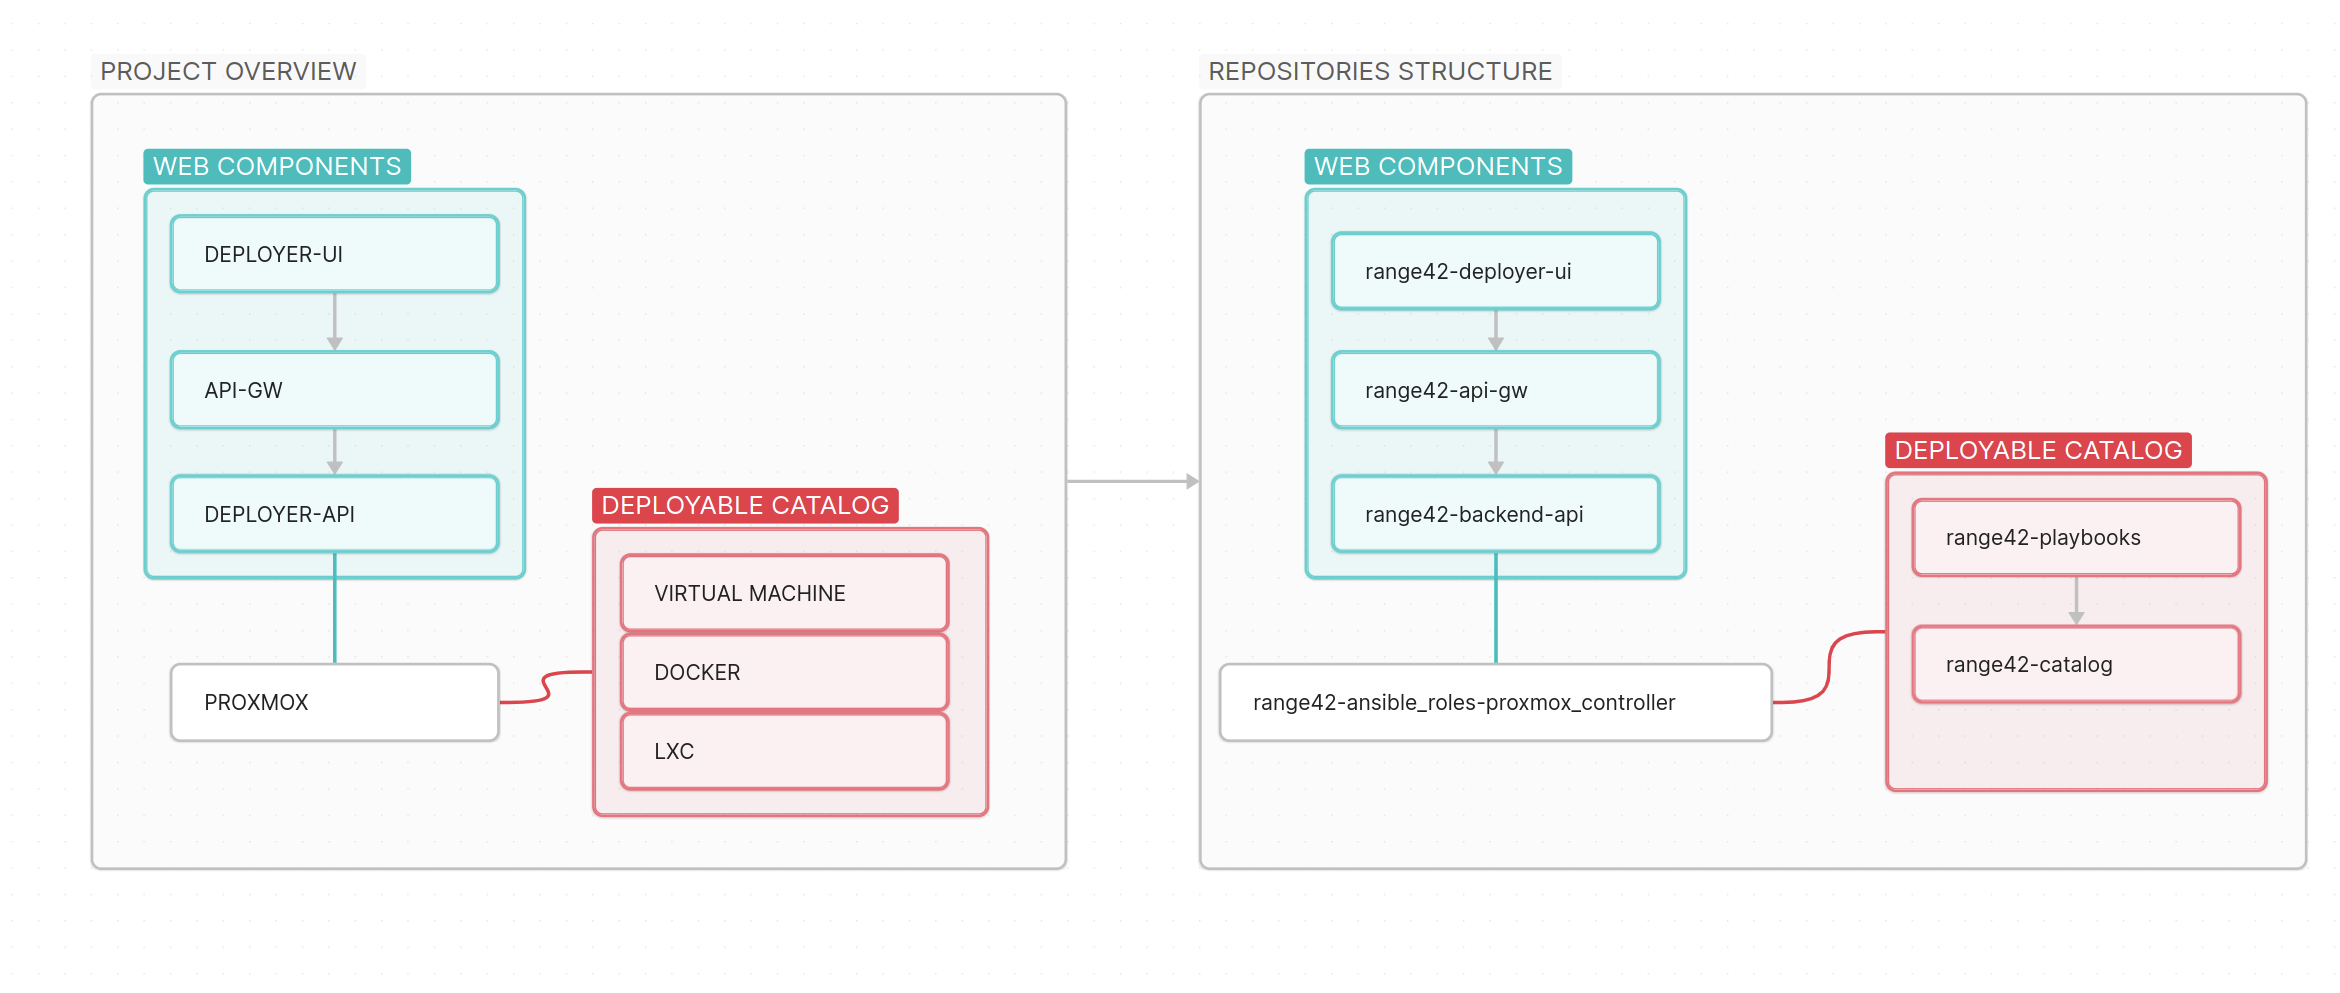
\includegraphics[width=0.95\textwidth]{../../images/diagrams/architecture.png}
  \end{figure}
  \vspace{-3mm}
  \begin{tcolorbox}
    \faInfoCircle\; \textbf{Gauche} : flux d'architecture logique. \textbf{Droite} : structure des d\'ep\^ots GitHub.
  \end{tcolorbox}
  \note[item]{Gauche = architecture logique ; droite = d\'ep\^ots GitHub r\'eels.}
\end{frame}

% === D\'EMO DEPLOYER UI ===
\section{D\'emo en direct : Deployer UI}

\begin{frame}{Deployer UI : concepteur visuel de labs \; \faDrawPolygon}
  \begin{columns}[T]
    \column{0.48\textwidth}
    \textbf{\faEdit\; Conception}
    \begin{itemize}
      \item Glisser-d\'eposer VMs, LXC, r\'eseaux, routeurs, pare-feu
      \item Configurer CPU, m\'emoire, disque, ISO par n\oe ud
      \item S\'election de templates Proxmox avec auto-remplissage
      \item Connecter les n\oe uds pour d\'efinir la topologie
    \end{itemize}

    \column{0.48\textwidth}
    \textbf{\faPlay\; D\'eploiement}
    \begin{itemize}
      \item R\'econciliation et validation pr\'e-d\'eploiement
      \item Ordre : r\'eseaux $\rightarrow$ routeurs $\rightarrow$ VMs $\rightarrow$ config $\rightarrow$ d\'emarrage
      \item Statut en temps r\'eel via WebSocket
      \item D\'emarrer, arr\^eter, red\'emarrer, supprimer depuis l'UI
    \end{itemize}
  \end{columns}
  \note[item]{Poser le contexte avant de basculer vers la d\'emo en direct.}
\end{frame}

\begin{frame}{D\'emo en direct \; \faPlay}
  \begin{center}
    {\Large \faDesktop\quad Basculer vers la d\'emo en direct}\\[8mm]
    \textbf{D\'eroulement de la d\'emo}\\[4mm]
    \begin{enumerate}
      \item Cr\'eer un nouveau projet sur le canvas
      \item Ajouter des VMs, r\'eseaux et un routeur
      \item Configurer les templates et les ressources
      \item D\'eployer sur Proxmox
      \item Observer les mises \`a jour de statut en temps r\'eel
      \item Contr\^oler les VMs depuis l'UI (d\'emarrage/arr\^et)
    \end{enumerate}
  \end{center}
  \note[item]{Slide de transition -- basculer vers le deployer UI ici.}
  \note[item]{D\'emo de 5 minutes max. Focus sur l'effet wow : conception $\rightarrow$ d\'eploiement $\rightarrow$ en direct.}
\end{frame}

% === MATURIT\'E DU BACKEND API ===
\begin{frame}{Backend API : pr\^et pour la production \; \faCogs}
  \begin{columns}[T]
    \column{0.48\textwidth}
    \textbf{Refactoring majeur}
    \begin{itemize}
      \item 86 fichiers de routes $\rightarrow$ \textbf{10 modules m\'etier}
      \item 52 fichiers de sch\'emas $\rightarrow$ modules regroup\'es
      \item Pattern application factory
      \item Logging structur\'e int\'egral
      \item Gestion centralis\'ee des secrets
    \end{itemize}

    \column{0.48\textwidth}
    \textbf{Nouvelles capacit\'es}
    \begin{itemize}
      \item \alert{D\'eploiement Docker} (compose)
      \item \alert{API WebSocket} pour le statut en direct
      \item \alert{Suite de tests} : unitaires + int\'egration
      \item \alert{Documentation Sphinx}
    \end{itemize}
  \end{columns}
  \note[item]{Le backend est pass\'e de la qualit\'e prototype \`a la qualit\'e production.}
\end{frame}

% === AUJOURD'HUI VS DEMAIN ===
\section{Aujourd'hui \& demain}

\begin{frame}{Aujourd'hui vs.\ demain}
  \begin{columns}[T]
    \column{0.48\textwidth}
    {\textbf{\faCheckCircle\; Op\'erationnel aujourd'hui}}
    \begin{itemize}
      \item Automatisation compl\`ete Proxmox (VMs, LXC, r\'eseau, pare-feu, VPN)
      \item Concepteur visuel de labs (glisser-d\'eposer)
      \item Statut VM en temps r\'eel via WebSocket
      \item Provisionnement par templates + r\'econciliation
      \item D\'eploiement API via Docker
      \item Monitoring Wazuh int\'egr\'e
    \end{itemize}

    \column{0.48\textwidth}
    {\textbf{\faRocket\; Prochaines \'etapes}}
    \begin{itemize}
      \item Plateforme de gestion d'exercices (notation \& rapports)
      \item G\'en\'eration de sc\'enarios assist\'ee par LLM
      \item Topologies multi-sous-r\'eseaux d'entreprise
      \item Moteur d'\'etat d\'eclaratif en direct (DLSE)
      \item Sc\'enarios ICS / IoT
      \item \'Echange f\'ed\'er\'e de catalogues
    \end{itemize}
  \end{columns}
  \note[item]{Gauche = op\'erationnel et d\'emontrable. Droite = en d\'eveloppement ou planifi\'e.}
\end{frame}

% === FEUILLE DE ROUTE : 6 AXES ===
\begin{frame}{Feuille de route : 6 axes strat\'egiques \; \faRoad}
  \small
  \begin{columns}[T]
    \column{0.48\textwidth}
    \textbf{Axe 0} -- Stabilisation \& durcissement\\
    {\footnotesize Verrouiller l'architecture, \'elargir le catalogue \`a 50+ labs}\\[2mm]
    \textbf{Axe 1} -- Gestion d'\'etat (DLSE)\\
    {\footnotesize Moteur d'\'etat d\'eclaratif pour la r\'econciliation}\\[2mm]
    \textbf{Axe 2} -- Interfaces utilisateur\\
    {\footnotesize Deployer UI, EMP avec tableaux de bord}

    \column{0.48\textwidth}
    \textbf{Axe 3} -- Services pour les \'etudiants\\
    {\footnotesize Portails, workflows guid\'es, acc\`es libre-service}\\[2mm]
    \textbf{Axe 4} -- Syst\`emes industriels \& IoT\\
    {\footnotesize Sc\'enarios d'entra\^inement ICS/SCADA et IoT}\\[2mm]
    \textbf{Axe 5} -- \'Ecosyst\`eme open source\\
    {\footnotesize Synergie NGSOTI, catalogues f\'ed\'er\'es, communaut\'e}
  \end{columns}
  \vspace{3mm}
  \begin{tcolorbox}
    \faInfoCircle\; Bas\'e sur le cadre d'ex\'ecution Range42 v0.8 -- 50 blocs de travail sur 6 axes avec s\'equencement trimestriel.
  \end{tcolorbox}
  \note[item]{Ces axes proviennent du cadre d'ex\'ecution officiel Range42 v0.8.}
\end{frame}

% === D\'EP\^OTS CL\'ES ===
\section{D\'ep\^ots cl\'es}

\begin{frame}{Vue d'ensemble de l'organisation \; \faClipboardCheck}
  \textbf{14 d\'ep\^ots} (10 publics, 4 priv\'es) -- \alert{520+ commits}, z\'ero vuln\'erabilit\'e critique\\[3mm]

  \begin{table}
    \footnotesize\color{cyber-ink}
    \begin{tabular}{l|ccl}
      \textbf{D\'ep\^ot} & \textbf{Commits} & \textbf{Langage} & \textbf{Statut} \\
      \hline
      backend-api & 156 & Python / FastAPI & Actif \\
      proxmox\_controller & 112 & Ansible / YAML & Actif \\
      catalog & 97 & Ansible / Docker & Stable \\
      playbooks & 81 & Ansible / YAML & Actif \\
      deployer-ui & 74 & Vue 3 / TypeScript & Actif \\
    \end{tabular}
  \end{table}
  \note[item]{Compteurs de commits \`a jour. Souligner la v\'elocit\'e du backend et du deployer-ui.}
\end{frame}

% === LE\c{C}ONS APPRISES ===
\section{Le\c{c}ons apprises}

\begin{frame}{Le\c{c}ons apprises \; \faLightbulb}
  \begin{columns}[T]
    \column{0.48\textwidth}
    \textbf{Technique}
    \begin{itemize}
      \item \alert{Ansible + API Proxmox} = combo IaC puissant
      \item Les snapshots sont essentiels pour les resets
      \item \alert{Refactorer t\^ot est payant} (86 $\rightarrow$ 10 fichiers de routes)
      \item WebSocket permet une UX temps r\'eel convaincante
    \end{itemize}

    \column{0.48\textwidth}
    \textbf{Processus}
    \begin{itemize}
      \item \alert{La gouvernance co\^ute du temps} mais d\'ebloque la collaboration
      \item Le cadre \`a 6 axes aligne une petite \'equipe
      \item La doc est toujours en retard sur le code
      \item Docker simplifie le d\'eploiement multi-environnement
    \end{itemize}
  \end{columns}
  \note[item]{\^Etre honn\^ete sur les d\'efis. Cela renforce la confiance du public.}
\end{frame}

% === D\'EFIS OUVERTS ===
\begin{frame}{D\'efis ouverts \& opportunit\'es \; \faExclamationTriangle}
  \begin{columns}[T]
    \column{0.48\textwidth}
    \textbf{Contenu \& couverture}
    \begin{itemize}
      \item \'Elargir \`a 50+ sc\'enarios d\'eployables
      \item Contenu ICS/IoT et forensique
      \item Format de sc\'enario standardis\'e
    \end{itemize}

    \column{0.48\textwidth}
    \textbf{Maturit\'e de la plateforme}
    \begin{itemize}
      \item CI/CD sur tous les d\'ep\^ots
      \item Plateforme de gestion d'exercices
      \item \'Echange f\'ed\'er\'e de catalogues (NGSOTI)
    \end{itemize}
  \end{columns}
  \vspace{3mm}
  \begin{tcolorbox}
    \faUsers\; \textbf{Votre expertise compte} : chaque contribution -- code, docs, tests, sc\'enarios -- fait avancer la plateforme.
  \end{tcolorbox}
  \note[item]{Pr\'esenter les d\'efis comme des opportunit\'es de contribution.}
\end{frame}

% === CONCLUSION ===
\begin{frame}{Participez \; \faRocket}
  \begin{columns}[T]
    \column{0.6\textwidth}
    \textbf{Contribuer}
    \begin{itemize}
      \item \textbf{Sc\'enarios} : recherche CVE, automatisation, gamification
      \item \textbf{Infrastructure} : r\^oles Ansible, backend API, CI/CD
      \item \textbf{UI/UX} : concepteur de labs, plateforme de gestion d'exercices
    \end{itemize}
    \vspace{3mm}
    \faGlobe\; \texttt{range42.lu} \quad \faGithub\; \texttt{github.com/range42}\\[1mm]
    \faEnvelope\; \texttt{info@nc3.lu}

    \column{0.35\textwidth}
    \begin{figure}
      \centering
      
\includegraphics[width=0.85\textwidth]{../../images/contribute.png}
    \end{figure}
  \end{columns}
  \vfill
  {\footnotesize \textcolor{white}{Compos\'e avec \LaTeX{}} {\textcolor{blue}{\faHeart}}}
  \note[item]{Appel \`a l'action final avec les prochaines \'etapes et les coordonn\'ees.}
\end{frame}

\end{document}
